
%References:
% latexdraw.com/how-to-use-the-foreach-loop-in-latex/
% overleaf.com/learn/latex/LaTeX_Graphics_using_TikZ%3A_A_Tutorial_for_Beginners_(Part_1)%E2%80%94Basic_Drawing

\documentclass[a4paper, 12pt, reqno]{amsart}

\usepackage[T1]{fontenc}
\usepackage[margin=3cm]{geometry}
\usepackage[parfill]{parskip}

%Line spacing
\usepackage{setspace}
\setstretch{1.25}

\usepackage{dsfont}
\usepackage{amsmath}
%\usepackage{natbib}

%Drawing vector grids
\usepackage{tikz}

\begin{document}
	This file outlines a possible method for proving that all 2 by 2 matrices modulo a prime power have a vector with maximal cycle length (a cycle length the same as the matrix's,
	the matrix's multiplicative order).
	
	Let $A = 
	\begin{bmatrix}
		\vec{v_1} & \vec{v_2}
	\end{bmatrix}$
	be a matrix with column vectors $\vec{v_1}, \vec{v_2} \in \mathds{Z}_{p^k}^2$ for some prime power $p^k$. We'll assume a smallest, nonzero $\omega$ exists such that 
	\[
		A^{\omega} \equiv I \mod{p^k}
	\]
	$\omega$ is then the cycle length of $A$.
	
	\emph{Case 1 - $A$ is invertible, and one of $\vec{v_1}$ or $\vec{v_2}$ has maximal cycle length} \\
	If either $\vec{v_1}$ or $\vec{v_2}$ already has maximal cycle length (that is, $\omega$ is the smallest nonzero number such that $A^{\omega}\vec{v_1} \equiv \vec{v_1}$
	or $A^{\omega}\vec{v_2} \equiv \vec{v_2}$), then we know for sure that $A$ has at least one vector of maximal cycle length.
	
	\emph{Case 2 - $A$ is invertible, and neither $\vec{v_1}$ nor $\vec{v_2}$ has maximal cycle length} \\
	If neither $\vec{v_1}$ nor $\vec{v_2}$ has maximal cycle length, then it must be the case that the two vectors' cycle lengths don't divide each other. Otherwise, if one of the
	cycle lengths did divide the other, then the larger of the two lengths would also be the cycle length of the matrix since both vectors would cycle back once the vector with
	the larger cycle length cycled. Thus, one of the vectors would have maximal cycle length, and we've already dealt with this case.
	
	Now, because the two cycle lengths don't divide each other, their cycle spaces cannot possibly span the entirety of $\mathds{Z}_{p^k}^2$. Why? The cycle space $S$ for a vector 
	$\vec{w}$ is defined as (when $A$ is invertible):
	\[
		S = \text{span}(\{\vec{w}, A\vec{w}, {A^2}\vec{w}, \cdots, {A^{\omega-1}}\vec{w}\})
	\]
	Essentially, the cycle space for a vector $\vec{w}$ is the set of all vectors which can be created as linear combinations of the iterations of $\vec{w}$ under $A$.
	
	All vectors in a vector's cycle space must have cycle lengths that divide the generating vector's cycle length. For instance, assume the vector $\vec{w}$ has a cycle length
	of 6. Every vector in the cycle space of $\vec{w}$ will take the form
	\[
		a_{0}\vec{w} + a_{1}A\vec{w} + a_{2}A^{2}\vec{w} + \cdots
	\]
	We know $\vec{w}$ has a cycle length of 6, so
	\begin{align*}
		          & A^{6}(a_{0}\vec{w} + a_{1}A\vec{w} + a_{2}A^{2}\vec{w} + \cdots)         \\
		\equiv \, & a_{0}A^{6}\vec{w} + a_{1}AA^{6}\vec{w} + a_{2}A^{2}A^{6}\vec{w} + \cdots \\
		\equiv \, & a_{0}\vec{w} + a_{1}A\vec{w} + a_{2}A^{2}\vec{w} + \cdots
	\end{align*}
	This shows that any vector within the cycle space of $\vec{w}$ must cycle whenever $\vec{w}$ cycles, so the cycle length of any vector within the cycle space must divide
	the cycle length of $\vec{w}$.
	
	Since, in this case, we know the cycle lengths of $\vec{v_1}$ and $\vec{v_2}$ don't divide each other, then there must be at least one vector in each cycle space that isn't
	in the other cycle space. This means that both the cycle space of $\vec{v_1}$ and the cycle space of $\vec{v_2}$ cannot span the entirety of $\mathds{Z}_{p^k}^2$.
	
	In fact, we can get a pretty good idea as to what the cycle spaces of each vector look like. We know the matrix $A$ is invertible, so at some point an iteration of $A$ will
	look like
	\[
		A^n \equiv 
		\begin{bmatrix}
			1 & 0 \\
			0 & 1
		\end{bmatrix} \mod{p^k}
	\]
	This means the cycle space of $\vec{v_1}$ must contain the basis vector $\vec{e_1}$ and the cycle space of $\vec{v_2}$ must contain the basis vector $\vec{e_2}$. Both 
	$\vec{e_1}$ and $\vec{e_2}$ will have "full spans" in their directions (meaning every multiple of $\vec{e_1}$ and $\vec{e_2}$ is unique). Therefore, for the two cycle spaces
	not to span the entirety of $\mathds{Z}_{p^k}^2$, it must be the case that $\vec{v_1}$ and $\vec{v_2}$ will look something like
	\[
		\vec{v_1} = 
		\begin{bmatrix}
			v_{11} \\
			pv_{12}
		\end{bmatrix}, \, \, \vec{v_2} = 
		\begin{bmatrix}
			pv_{21} \\
			v_{22}
		\end{bmatrix}
	\]
	where each vector's component corresponding to the direction perpendicular to the basis vector within their cycle space has a factor of $p$ attached to it. Otherwise, each 
	vector and its corresponding basis vector would be enough to span the entire module, which we know it can't. 
	
	Because of this, we know that both column vectors in $A$ have cycle spaces that are composed of parallel lines of vectors, each a power of $p$ apart. For mod $p^3$ and above,
	there's some variation as to how this arrangement will look. For $p^2$, however, there's only one power of $p$ to use to separate these lines: $p^1$. Below is a visual for what
	the cycle spaces of $\vec{v_1}$ and $\vec{v_2}$ will look like mod $5^2$. 
	
	\begin{figure}[b]
		\centering
		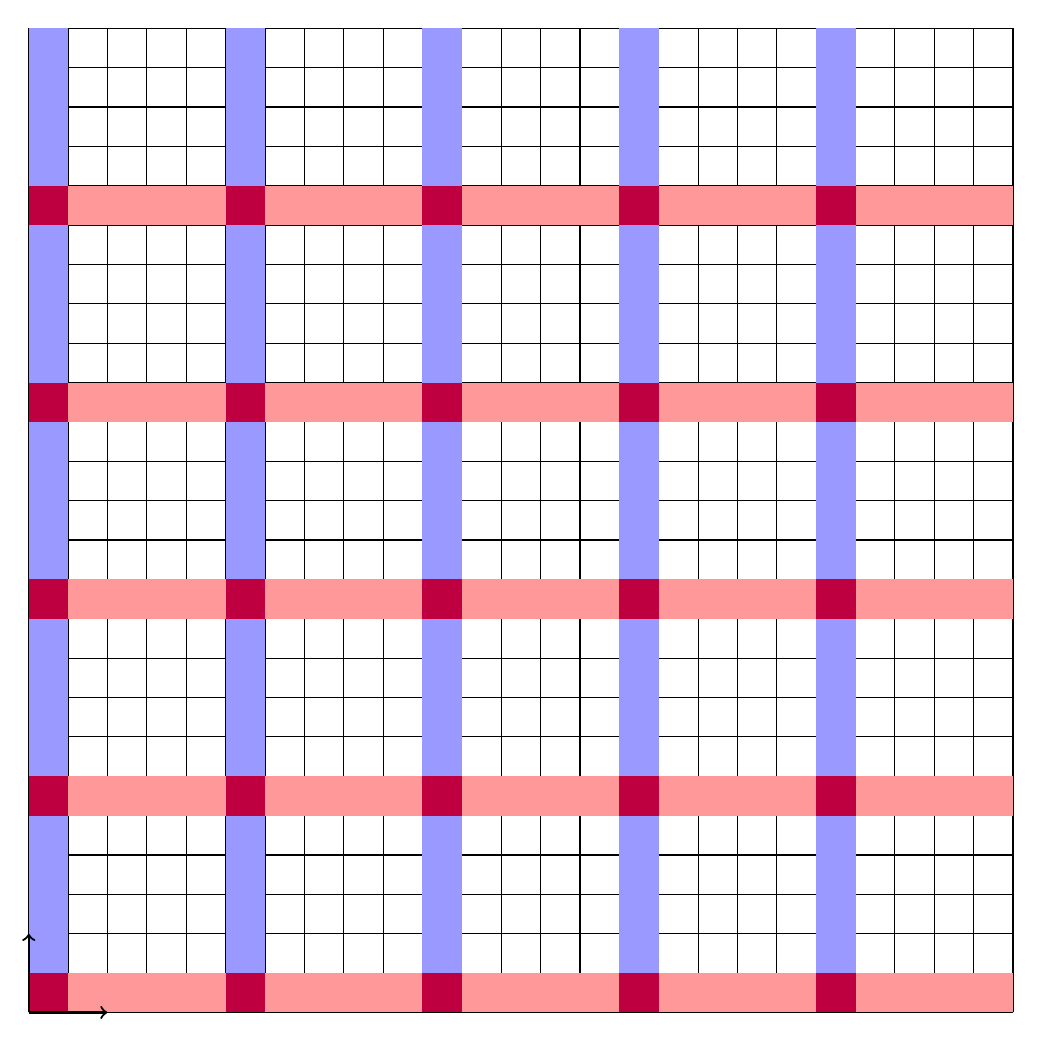
\begin{tikzpicture}
			%Vector grid
			\draw[step=0.5cm, black, thin] (0, 0) grid (12.5, 12.5);
			
			\foreach \i in {0, 2.5, ..., 10}
			{
				%v_1's cycle space
				\fill[red!40!white] (0, \i) rectangle (12.5, \i+0.5);
				
				%v_2's cycle space
				\fill[blue!40!white] (\i, 0) rectangle (\i+0.5, 12.5);
			}
			
			%Shared vectors
			\foreach \i in {0, 2.5, ..., 10}
			{
				\foreach \j in {0, 2.5, ..., 10}
				{
					\fill[purple] (\i, \j) rectangle (\i+0.5, \j+0.5);
				}
			}
			
			%Axes
			\draw[thick, ->] (0, 0) -- (1, 0);
			\draw[thick, ->] (0, 0) -- (0, 1);
		\end{tikzpicture}
		\caption{Visual of cycle spaces for $\vec{v_1}$ and $\vec{v_2}$ mod $5^2$. The cycle space of $\vec{v_1}$ is coloured red while the cycle space of $\vec{v_2}$ is
		coloured blue. Vectors which are shared between them are coloured purple. The bottom-left square is $\vec{0}$.}
	\end{figure}
	
	Okay, so the cycle spaces of $\vec{v_1}$ and $\vec{v_2}$ don't span $\mathds{Z}_{p^k}^2$. However, there must be at least one vector whose cycle space \emph{does} span
	$\mathds{Z}_{p^k}^2$. How do we know this? Let's first consider the prime case. In $\mathds{Z}_{p}^2$, the only way for an invertible matrix to not have a vector whose cycle
	space spans the module is if all vectors stay on their initial spans. In other words, the action of $A$ would be to simply scale all vectors by some constant:
	\[
		A\vec{w} \equiv \lambda\vec{w} \,\, \text{for all $\vec{w}$} \mod{p}
	\]
	
	Shuffling this around a bit:
	
	\begin{align*}
		         & A\vec{w} - \lambda\vec{w} \equiv \vec{0} \\
		\implies & (A - \lambda I)\vec{w} \equiv \vec{0}
	\end{align*}
	This statement must be true for all $\vec{w}$, so the matrix must be zero:
	\begin{align*}
		         & A - \lambda I \equiv 0 \\
		\implies & A \equiv \lambda I
	\end{align*}
	
	The only types of matrices in which this could happen are multiples of the identity matrix, and these matrices would be dealt with in case 1. It's important to note here that, 
	for the types of matrices we're dealing with in this case (case 2), it's impossible for a prime-powered matrix to reduce to a multiple of the identity mod the prime itself. This 
	is because the cycle lengths (multiplicative orders) of matrices must either stay the same or go up by a factor of $p$ when increasing the power of the prime modulus. The column 
	vectors in a scaled identity matrix would necessarily have the same cycle length, and when lifted to a prime-powered modulus, their cycle lengths would either stay the same--and 
	we'd be in case 1--or one of the cycle lengths would have to divide the other. Since the cycle length of the matrix would increase by $p$ in this case, one (or both) of the 
	column vectors would have to add a factor of $p$ to their cycle lengths to compensate, and this would put us, again, in case 1 since one of the cycle lengths would have to 
	divide the other.
	
	This means that, whenever we're dealing with a matrix that falls into this case (case 2), its reduction mod $p$ will have at least one vector whose cycle space spans
	$\mathds{Z}_{p}^2$, since there will be at least one vector that gets knocked off its span after an iteration by the matrix. However, this same vector's cycle space, when
	raised to a prime-powered modulus, will also necessarily span the module (since the basis vectors for the cycle space will continue to be linearly-independent when lifted to
	the prime-powered modulus).
	
	For any given matrix in case 2 under a prime-powered modulus $p^k$, there will necessarily be at least one vector whose cycle space spans $\mathds{Z}_{p^k}^2$. As we've stated
	before, all vectors in a vector's cycle space must have cycle lengths that divide the generating vector's cycle length. Because both $\vec{v_1}$ and $\vec{v_2}$ will
	necessarily be in this vector's cycle space, this means the cycle length of this vector must be a multiple of both the cycle length of $\vec{v_1}$ and $\vec{v_2}$. The smallest
	possible value that does this is the LCM of the two values, which is also the maximal cycle length for the matrix. Therefore, the vector whose cycle space spans the entire
	module will also have maximal cycle length, and a vector of this kind is guaranteed to exist for matrices which fall into this case.
	
	\emph{Case 3 - A isn't invertible} \\
	If our starting matrix $A$ isn't invertible, we can instead look at the module restricted to the core of this matrix. The core of a matrix is the largest set of vectors $S$
	for which
	\[
		AS = S
	\]
	meaning $A$ is invertible over the set $S$. If my previous ideas on the cores of matrices mod some prime power are correct (the stuff from "Exploring matrix cores within
	prime-powered modules"), then the cores of matrices under prime-powered moduli should always have a linearly-independent basis, meaning they can be treated as if they were
	any other matrix system. If this is indeed the case, then the behaviour of the matrices' cores should be encapsulated in cases 1 and 2 from above.
	
	If the things on this file are correct, then for all 2 by 2 matrices mod a prime-power, there should be at least one vector of maximal cycle length.
\end{document}
